
\section{Background theory}

\subsection{Mathematical model (Quasi-steady )}

 One of the widely used mathematical model to predict the system response under galloping is the Quasi-steady state (QSS) model, incorporated by \cite{Parkinson1964} for a square cross section. The equation of motion of the body under galloping is given by Eq. \eqref{equationofmotion}. The forcing term $F_y$ is given by Eq.\eqref{lift equation}.
 
 \begin{figure}
\centering
\includegraphics[width=0.5\linewidth]{../FnP/setup_1}
\caption{}
\label{fig:setup_1}
\end{figure}


\begin{equation}
\label{equationofmotion}
(m+m_a)\ddot{y}+c\dot{y}+ky=F_y
\end{equation}

\begin{equation}
\label{lift equation}
F_y=\frac{1}{2}\rho U^2C_y
\end{equation}

 In the QSS  model $C_y$ is determined by an interpolating polynomial based on the stationary lift and drag data. The order of the interpolation polynomial has varied from study to study (e.g..$7^{th}$ order was used in \cite{Parkinson1964} and $3^{rd}$ order polynomial was used in \cite{Barrero-Gil2009}. \cite{Ng2005} concluded that using a $7^{th}$ order polynomial is sufficient and a polynomial higher than that of $7^{th}$ order polynomial neither results in a result significantly better result nor does it exhibit an additional amplitudes of oscillation. Thus A $7 ^{th}$ order interpolating polynomial is incorporated in this present study. 

\begin{equation}
\label{cy ploynomial}
C_y(\alpha)=a_1\left(\frac{\dot{y}}{U}\right)+a_3\left(\frac{\dot{y}}{U}\right)^3+a_5\left(\frac{\dot{y}}{U}\right)^5+a_7\left(\frac{\dot{y}}{U}\right)^7
\end{equation}

%\begin{equation}
%\label{modified_equation_of_motion}
%\ddot{y}+c^*\dot{y}+k^*y=\frac{1}{2}\rho U^2A
%\end{equation}

\cite{Joly2012} used a sinusoidal forcing function to the RHS of the oscillator model (Eq. \eqref{equationofmotion}) in order to represent forcing due to VIV. This method provided satisfactory results with the numerical simulations obtained at low mass ratios. This study, the forcing due to VIV is incorporated using a sinusoidal forcing function $F_0\sin{\omega_{s}t}$ added to the RHS. $\omega_{s}$ and $F_0$ represents shedding frequency and the maximum force due to shedding respectively. Thus, the final equation is represented by Eq. \eqref{final_equation_motion}.    

\begin{equation}
\label{final_equation_motion}
(m{+}m_a)\ddot{y}{+}c{+}\dot{y}{+}ky{=}\frac{1}{2}\rho U^2 \text{A} \Bigg(a_1\left(\frac{\dot{y}}{U}\right){+}a_3\left(\frac{\dot{y}}{U}\right)^3{+}a_5\left(\frac{\dot{y}}{U}\right)^5{+}a_7\left(\frac{\dot{y}}{U}\right)^7 \Bigg){+} F_0\sin{(\omega_s t)}
\end{equation}

This equation could be solved by time integration methods. In  this study  ``Ode 45" routine in MATLAB was used to obtain the solutions.

\subsection{Calculation of average power}

 The dissipated power due to the damper could be expressed as the harvested power output assuming that the other  power dissipation due to internal damping such as friction of the system is negligible. Therefore the mean power output could be given by Eq. \eqref{power}. 
  
 
 \begin{equation}
 \label{power}
P_{mean}=\frac{1}{T}\int_{0}^{T}(c\dot{y})\dot{y} dt
 \end{equation}
 
\subsection{Parameters used} 
 
The stationary data and the FSI data were obtained using a higher order spectral element code which simulates 2D laminar flow. The Reynolds number was kept at 165 as it was pointed out by \cite{Sheard2009} and \cite{Tong2008} that the 3 dimensional transition for a square cylinder occurs at approximately Re-160. $F_0$ was kept at $0.4937$ which was obtained by using a simple linear interpolation on the data of \cite{Joly2012}. $\omega_s$ was set to $0.98$ winch was obtained by a power spectral analysis of the stationary data at $0^0$. Stationary $C_y$ data were obtained at different angles of attack ranging from $0^0$ to $16^0$. The average power was obtained by using Eq. \eqref{power} with data sets consisting substantial amount of peaks. In order to obtain a comparison with high Reynolds number power data was obtained using \cite{Parkinson1964} $C_y$ data.


 FSI data were obtained for the oscillating (free-vibration) scenario. The Naiver-Stokes equations were solved using an accelerated frame of reference using the previously mentioned code. A three-step time splitting scheme together with high-order Lagrangian polynomials were used to obtain the solution. The details of the method could be found in \cite{Thompson2006,Thompson1996a}. This code was incorporated in \cite{Leontini2011,Leontini2007a}  where it was employed in a fluid-structure interaction problems. 
 
 The computational domain consists of 690 quadrilateral macro elements(refer figure) where majority of the elements were concentrated near the square section. A freestream condition was given to the inlet, top and bottom boundaries and the normal velocity gradient was set to zero at the outlet. A convergence study was performed by changing the order of the polynomial ($p$-refinement) at $U^*=40$ and Re $165$. A 9th order polynomial together with a time step of $\frac{\Delta tU}{D}=0.001$ was sufficient to ensure an accuracy of $2\%$ with regards to amplitude of oscillation.  
 
\begin{figure}

  \setlength{\unitlength}{\textwidth}
  \begin{picture}(1,0.3)(0,0.8)
    
    % % %90
      \put(0.025,0.9){\includegraphics[width=0.5\unitlength]{../FnP/gnuplot/lift_curve_165.eps}}
      \put(0.495,0.9){\includegraphics[width=0.5\unitlength]{../FnP/gnuplot/lift_curve_park.eps}}
     
   
	
            
      
      
   
 	\put(-0.01,1.02){ $c_y$} 	
% 	\put(0.56,1.02){ $\theta$}
 	
 	 	\put(0.25,0.88){ $\theta$} 	
 	 	\put(0.75,0.88){ $\theta$}



    \put(0.09,0.88){(a)}
    \put(0.56,0.88){(b)}
   
       

  \end{picture}

  \caption{Lift coefficient, $C_y$, as a function of incidence angle $\theta$, for a static square cross section at Re=165 by(a). Points ($\bullet$) are measurements from simulations.The data obtained by \cite{Parkinson1964} at Re=22300 are represented by (b). The solid line is a 7th-order polynomial fit that has been used to calculate the right-hand side of equation 4 throughout this study}
    \label{fig:lift_curves}
\end{figure}
 
 
 

 
 
 
 









